\documentclass[report,dvipdfmx]{jlreq}
\usepackage{graphicx}
\usepackage[version=4]{mhchem}
\usepackage{cite}
\usepackage{amsmath}
\usepackage{mathtools}
\usepackage{textcomp}
% \usepackage{caption}
\usepackage{subcaption}
% \usepackage{amssymb}
\usepackage{url}

\includeonly{
    % master_thesis_contents/master_thesis_goto_0abstract.tex,
    master_thesis_contents/master_thesis_goto_1intro.tex,
    master_thesis_contents/master_thesis_goto_2mmobs.tex,
    master_thesis_contents/master_thesis_goto_3mm_analysis.tex,
    % master_thesis_contents/master_thesis_goto_4results.tex,
    % master_thesis_contents/master_thesis_goto_5discussion.tex,
    % master_thesis_contents/master_thesis_goto_6conclusion.tex,
    % master_thesis_contents/master_thesis_goto_7ack.tex,
    % master_thesis_contents/master_thesis_goto_app1sofie.tex,
    % master_thesis_contents/master_thesis_goto_app2poes.tex
}

\begin{document}

\title{ミリ波分光計を用いた北極域・南極域における \\ 中層大気中の一酸化窒素分子変動の観測的研究}
% \title{北極域・南極域における中層大気中の \\ 一酸化窒素分子の大気観測および柱密度変動と \\ 高エネルギー電子の降り込みの解析}
\author{名古屋大学大学院工学研究科電気工学専攻 \\ 後藤宏文}
\date{\empty}

\maketitle

% abstract
\begin{abstract}
    abstract
    % 概要を書く
\end{abstract}


\tableofcontents

% \chapter{イントロダクション}
\chapter{イントロダクション}
\label{ch:intro}
\ref{ch:intro}章では我々が行う研究の背景について述べる。
まず\ref{sec:intro_background}節では地球大気でのオゾンの重要性と高エネルギー粒子の降り込みとオゾンの減少について述べる。
次に\ref{sec:intro_privious}節では、先行研究で明らかになったことと、問題点について述べる。
最後に\ref{sec:intro_porpose}節では\ref{sec:intro_privious}節の内容を踏まえて本研究の目的について述べていく。


\section{研究背景}
\label{sec:intro_background}
% \begin{itemize}
%     \item 高エネルギー粒子のモデル結果と観測結果の差を示す
%     \item EPPからO3の現象までの流れを示す
% \end{itemize}
% ここでNOの略称を紹介し、以後NOと略す
地球大気の大部分は窒素分子\ce{N2}と酸素分子\ce{O2}で占められているが、大気微量成分と呼ばれる\ce{N2}と\ce{O2}以外の大気分子も地球環境に影響を与えている。
オゾン分子\ce{O3}もその大気微量成分の1つであり、\ce{O3}の変動によって大気の放射バランスが変わり、地上の気候や気象に影響を与える可能性が指摘されている~\cite{rozanov2012influence,seppala2009geomagnetic}。
これまで、冷媒などに用いられたフロンガスなど人為的な原因によるオゾンの変動に着目した研究は行われてきた。
しかし、自然現象による原因の中でも、とくに太陽活動に伴う高エネルギー粒子の降り込み(EPP: Energetic Particle Precipitation)の影響によるオゾンの変動に関してシミュレーション結果と観測結果には大きな開きがあるため、十分な観測的理解には達していない(図\ref{fig:rozanov2012_seppala2009})。
\begin{figure}[htbp]
    \centering
    \begin{minipage}{\linewidth}
        \centering
        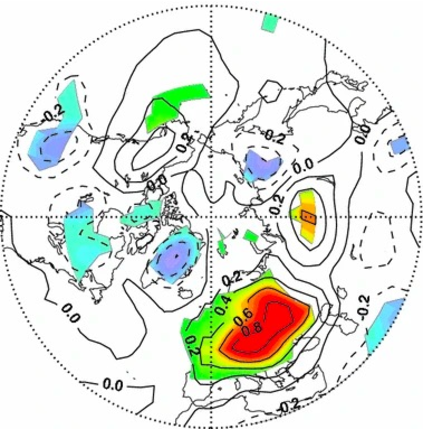
\includegraphics[scale=0.6]{master_thesis_contents/master_thesis_fig/rozanov2012_fig12.pdf}
        \subcaption{シミュレーション結果(最大で$0.8\, \mathrm{K}$の増加、~\cite{rozanov2012influence}より引用)}
        \label{fig:rozanov2012_fig12}
    \end{minipage}
    \begin{minipage}{\linewidth}
        \centering
        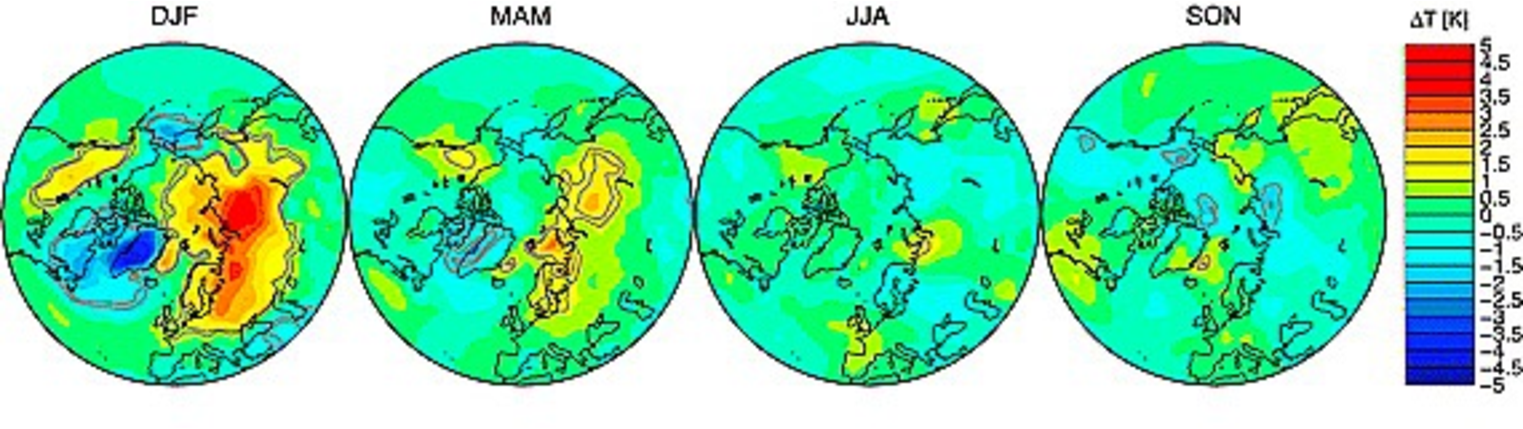
\includegraphics[scale=0.6]{master_thesis_contents/master_thesis_fig/seppala2009_fig3.pdf}
        \subcaption{観測データに基づいた統計結果(最大で$5\, \mathrm{K}$の増加、~\cite{seppala2009geomagnetic}より引用)}
        \label{fig:seppala2009_fig3}
    \end{minipage}
    \caption{EPP時の地表温度の変化$\Delta T\, \mathrm{[K]}$}
    \label{fig:rozanov2012_seppala2009}
\end{figure}
そこで我々の研究グループでは、EPPの影響によるオゾンの変動を観測的に明らかにすることを研究目的の1つとして研究を行っている。
EPPの影響によってオゾンの変動に影響を与えるまでには、図\ref{fig:epp_to_ozone_flow}のような流れで起きる。
\begin{figure}[htbp]
    \centering
    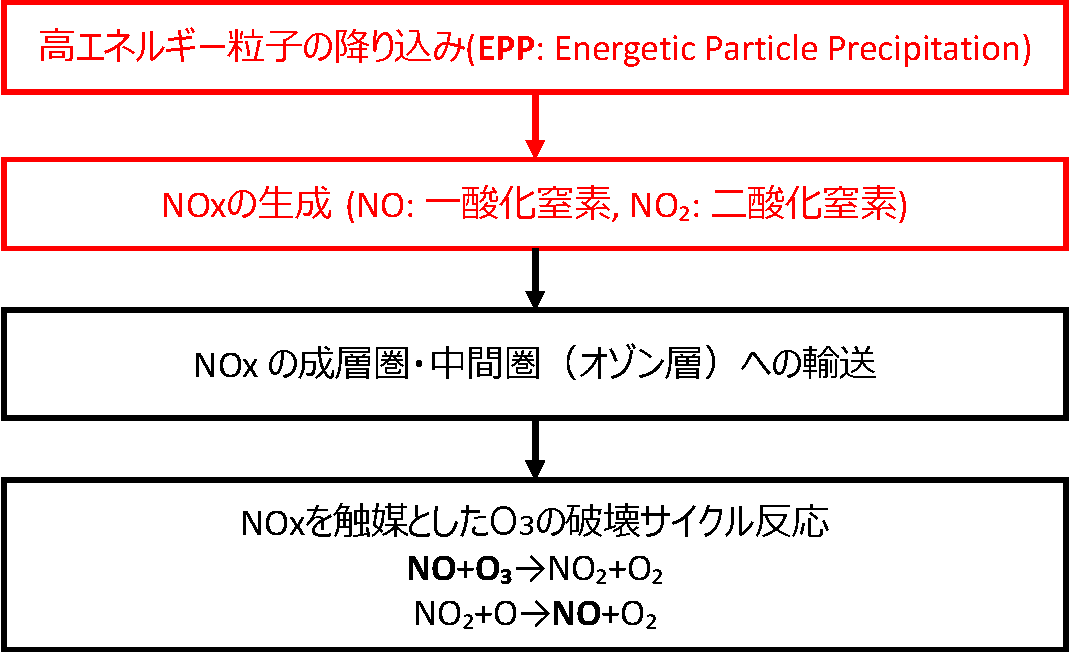
\includegraphics[width=\linewidth]{master_thesis_contents/master_thesis_fig/epp_to_ozone_flow.pdf}
    \caption{EPPからオゾン破壊までのフロー}
    \label{fig:epp_to_ozone_flow}
\end{figure}
まずEPPがあると、それによって\ce{NOx}と呼ばれる一酸化窒素\ce{NO}や二酸化窒素\ce{NO2}が生成される。
それが大気の輸送によって成層圏・中間圏に輸送されることにより、これらの反応式で表されるように\ce{O3}の破壊サイクル反応を起こす。


\section{先行研究の結果と課題}
\label{sec:intro_privious}
% \begin{itemize}
%     \item 衛星観測で示されたNOとO3の変動
%     \item ミリ波観測で示されたNOの短期変動と季節変動
%     \item 衛星観測では同じ場所での連続的な現象の観測が難しいこと
%     \item 衛星観測では、緯度方向にでしか議論が行われていないこと
%     \item ミリ波では夏に短期変動の観測ができないことを示す(観測手法でのトロムソの話につながる)
% \end{itemize}
先行研究では高エネルギー粒子の降込みによって\ce{NOx}が増加し、それがオゾンの変動に影響を与えていることが衛星観測のデータにて時間分解能が1日ではあるが示されている(図\ref{fig:lopez2005observation_fig3})~\cite{lopez2005observation}。
2003年10月28日にEPPがあったが、それと前後して\ce{NOx}の増加が確認されており、\ce{NOx}の増加があった地域に\ce{O3}の減少が確認されている。
\begin{figure}[htbp]
    \centering
    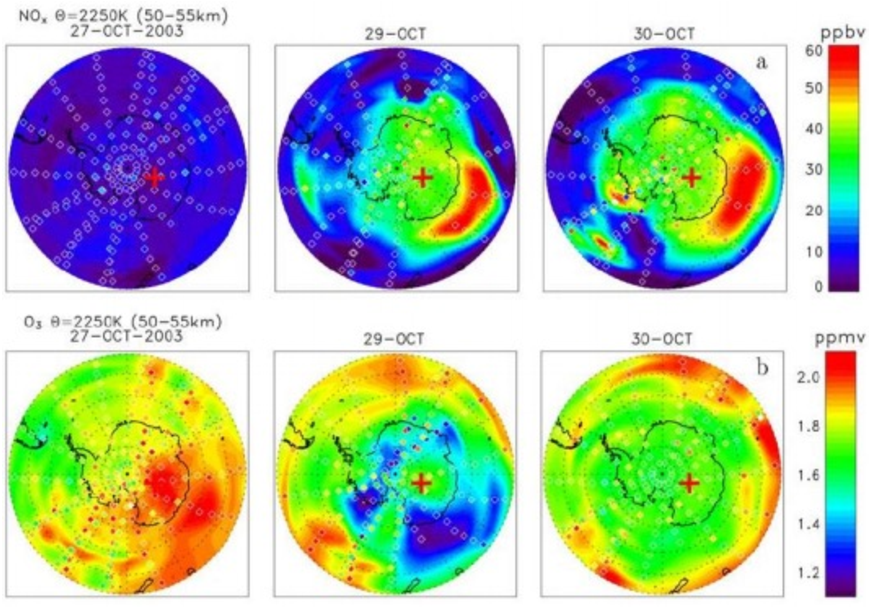
\includegraphics[width=\linewidth]{master_thesis_contents/master_thesis_fig/lopez2005observation_fig3.pdf}
    \caption{EPPイベントの前後での\ce{NOx}と\ce{O3}の変動(~\cite{lopez2005observation}より引用)}
    \label{fig:lopez2005observation_fig3}
\end{figure}
このように衛星観測では全球的な観測を行うことが可能ではあるが、時間分解能は比較的悪く、定点で連続的な現象の観測が難しいという課題がある。
その課題を克服するため、我々の研究グループではミリ波分光計(観測手法の詳細は\ref{ch:mm_obs}章)を用いた観測を行っている。


次に我々の研究グループで行われたミリ波分光計を用いた先行研究について話していく。
我々のグループでは2011年から南極昭和基地でミリ波分光による地上観測を行っている。
図\ref{fig:isono2014ground_fig5a}は2012年から2013年までの観測による解析結果である。
横軸が時系列になっていて月ごとに目盛りがふってあり、横軸において、黒色のエラーバーは\ce{NO}の存在量(厳密には柱密度。詳細は\ref{sec:derive_columndensity}節)を表している。
紫色の影の部分に関しては、それぞれの日で太陽が当たっていない時間を表している。
この結果より、季節にともなう長期的変動、冬には高エネルギー粒子によるものと考えられる短期変動が確認できた。
しかし、夏は太陽光による光解離の影響もあり高エネルギー粒子による影響と切り分けをすることができなかった。
\begin{figure}[htbp]
    \centering
    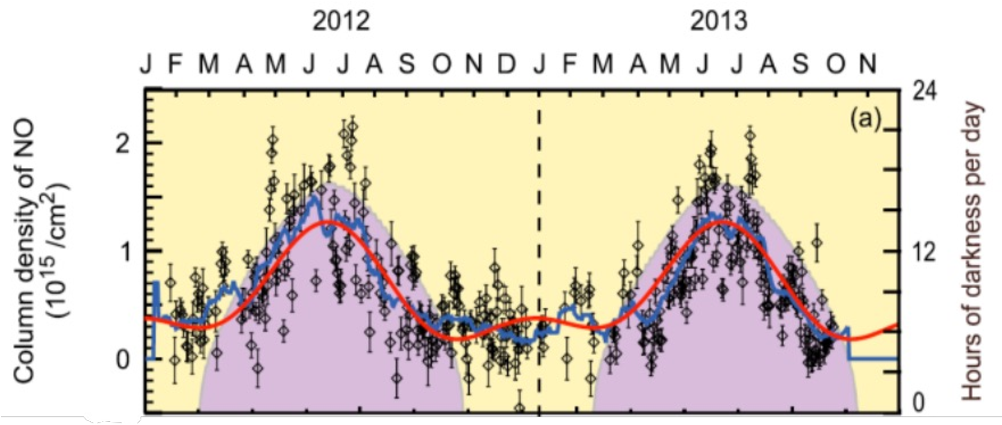
\includegraphics[width=\linewidth]{master_thesis_contents/master_thesis_fig/isono2014ground_fig5a.pdf}
    \caption{ミリ波分光計を用いた観測による南極・昭和基地での\ce{NO}の変動(~\cite{isono2014ground}より引用)}
    \label{fig:isono2014ground_fig5a}
\end{figure}
以上のことを踏まえて衛星観測とミリ波分光での地上観測による先行研究で明らかになったことと課題点についてまとめる。
\clearpage
\begin{itemize}
    \item 明らかになった点
    \begin{itemize}
        \item ミリ波分光を用いた地上観測(南極・昭和基地)
        \begin{itemize}
            \item 季節にともなう\ce{NO}の長期的変動
            \item EPPに伴う\ce{NO}の増加
        \end{itemize}
        \item 衛星観測
        \begin{itemize}
            \item EPPに伴う\ce{NO}の増加
            \item \ce{NO}の増加した地域にて見られた\ce{O3}の減少
        \end{itemize}
    \end{itemize}
    \item 課題点
    \begin{itemize}
        \item ミリ波分光を用いた地上観測(南極・昭和基地)
        \begin{itemize}
            \item 夏の\ce{NO}の短期変動の確認が難しい
        \end{itemize}
        \item 衛星観測
        \begin{itemize}
            \item 定点での連続的な観測が難しい
        \end{itemize}
    \end{itemize}
\end{itemize}
\ref{sec:intro_porpose}節では、これらの課題点を踏まえた本研究の目的について述べていく。


\section{本研究の目的と内容}
\label{sec:intro_porpose}
% \begin{itemize}
%     \item EPPからO3の現象までの流れの中でどこまでを扱うかを示す
% \end{itemize}
本研究では図\ref{fig:epp_to_ozone_flow}で示したフローの中でも上2つの関係について注目した(図\ref{fig:flow_and_porpose}中の赤枠)。
EPPについて、Dst指数と呼ばれる地磁気擾乱の大きさを表す指数と衛星観測による電子フラックスデータ、\ce{NOx}についてはミリ波観測による\ce{NO}スペクトルデータから導出した柱密度(柱密度の導出までの手法の詳細は\ref{ch:mm_analysis}章)をもとにして、お互いの関係性について調べることを研究目的としている。
\begin{figure}[htbp]
    \centering
    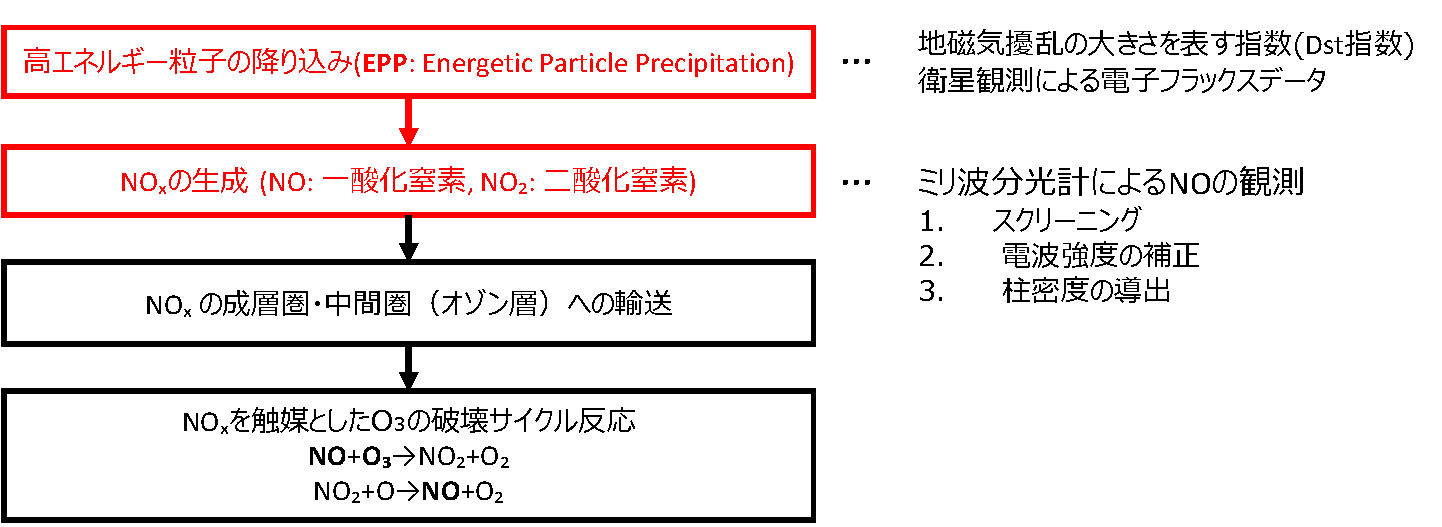
\includegraphics[width=\linewidth]{master_thesis_contents/master_thesis_fig/flow_and_porpose.pdf}
    \caption{図\ref{fig:epp_to_ozone_flow}と本研究の目的との対応}
    \label{fig:flow_and_porpose}
\end{figure}


% \chapter{ミリ波観測手法}
\chapter{ミリ波観測手法}
\label{ch:mm_obs}

\ref{ch:mm_obs}章では我々が用いるミリ波分光を用いた観測手法について述べる。
まず\ref{sec:mm_obs}節では観測手法について、また観測された電波強度に対して黒体を用いたキャリブレーション手法と、分子スペクトルを抽出するために行う電波強度の補正に用いる周波数スイッチングと、光学的厚みの測定について述べていく。
次にそれぞれの観測場所で用いられた分光計において、\ref{sec:mm_tromsoe}節でノルウェー・トロムソ(Troms\o , Norway)、\ref{sec:mm_syowa}節で南極・昭和基地(Syowa, Antarctic)について述べていく。

\section{観測手法}
\label{sec:mm_obs}

最初にミリ波分光を用いた観測手法について述べる。
私たちのグループでは、観測の手法としてミリ波電波分光法による地上観測を用いて大気分子を観測している~\cite{mizuno2002millimeter}。
その模式図を図\ref{fig:spectrometer_schema}に示す。
\begin{figure}[htbp]
    \centering
    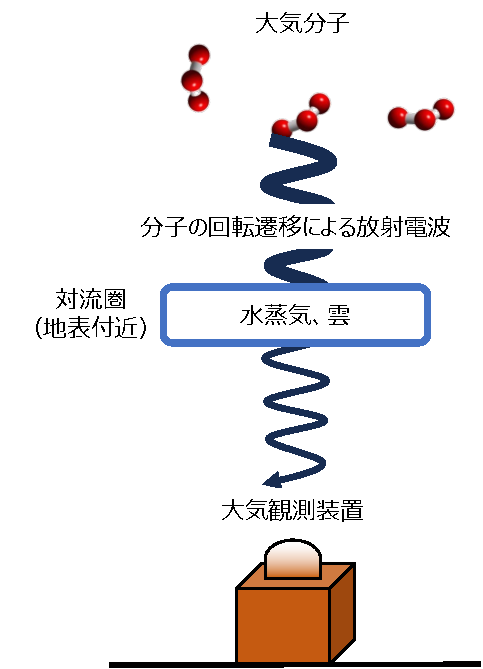
\includegraphics{master_thesis_contents/master_thesis_fig/spectrometer_schema.pdf}
    \caption{ミリ波電波分光法による地上観測の模式図}
    \label{fig:spectrometer_schema}
\end{figure}
ミリ波電波分光法では、観測対象の大気分子の回転遷移によって放射されるミリ波帯電波を受信し分光することで、電波放射スペクトルを観測している。
しかし、図\ref{fig:spectrometer_schema}に示す通りに電波を地上観測する上で下層大気の水蒸気や雲の影響を考慮する必要があり、そのために光学的厚みを計算する。
およそ5分間隔の積分時間で大気分子スペクトルを観測し、その5分の間隔の間に光学的厚みを測定している。
% 間隔時間はトロムソと昭和で一緒?
光学的厚みの測定方法の詳細は後述する。
ミリ波大気観測装置の概略図を図\ref{fig:mm_component}に示し、南極・昭和基地にて実際に設置されたミリ波分光計の様子を図\ref{fig:mmobs_spectrometer_syowa}に示す。
図\ref{fig:spectrometer_schema}に示すように観測装置は主に4つの部分に分かれている。
\begin{figure}[htbp]
    \centering
    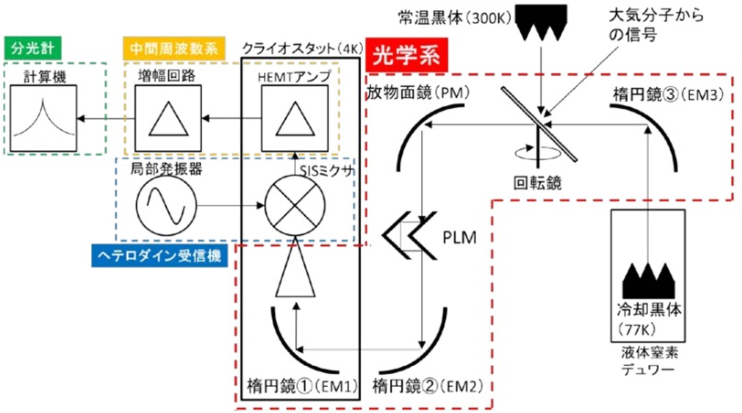
\includegraphics[width=\linewidth]{master_thesis_contents/master_thesis_fig/mm_component.pdf}
    \caption{ミリ波大気観測装置の概略図(~\cite{ito2017master}より引用)}
    % \caption{$\scriptstyle \mbox{ミリ波大気観測装置の概略図}\atop \scriptstyle \mbox{text}(~\cite{ito2017master}より引用$}
    \label{fig:mm_component}
\end{figure}
\begin{figure}[htbp]
    \centering
    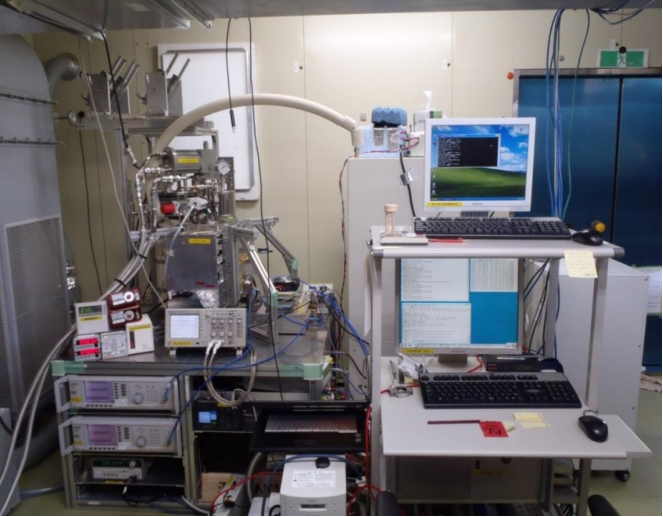
\includegraphics[width=\linewidth]{master_thesis_contents/master_thesis_fig/mmobs_spectrometer_syowa.pdf}
    \caption{南極の昭和基地に設置された観測装置(~\cite{uemura2014master}より引用)}
    \label{fig:mmobs_spectrometer_syowa}
\end{figure}
\begin{enumerate}
    \item 光学系 \mbox{} \\
        大気分子からの電波と、電波強度から黒体温度に変換する(詳細は後述)際に用いる常温黒体と冷却黒体からの電波を受信機内部まで集光し伝送する。
        また、回転鏡を用いることにより、大気観測における観測天頂角を変えることで光学的厚みの測定(詳細は後述)を行っている
    \item ヘテロダイン受信機 \mbox{} \\
        大気分子からの信号を局部発振器からの信号をミクサで混合している。
        大気分子からの電波は微弱であり、信号処理に適切なレベルまで増幅しなければならない。
        しかし、本研究で扱う電波の周波数(数百$GHz$程度)を直接増幅できる増幅器は実用レベルでは存在しない。
        そこで、観測装置で受信した信号をいったん低い周波数に下げることにより増幅する方法をとっている。
    \item 中間周波数系 \mbox{} \\
        低周波に変換された信号を分光計に適切な周波数にさらに変換し、分光計に必要なレベルまで増幅する。
    \item 分光計 \mbox{} \\
        デジタル高速フーリエ変換により分光処理を行い、大気分子のスペクトルを得る。
        入力信号を直接A/D変換して時系列データとして読み込み、それを高速フーリエ変換することにより周波数スペクトルを得ている。
        本研究で用いるデータを得るために用いられた分光計は16348チャンネルの周波数スペクトルデータを出力する~\cite{ito2017master}。
        % 昭和基地の場合のチャンネル数は?引用元をみないといけない
\end{enumerate}
ミリ波電波分光法による地上観測による利点は、太陽光などの背景光源を必要とせず昼夜モニタリングが可能となることである。
昼夜だけでなく白夜や極夜がある極地においても、その影響を受けずに連続観測することができる。
以上より、連続的・長期的に観測を行うことが可能で、自然起源や人為起源による長期的変動や短期的変動を観測することが可能であり、これが我々の研究グループでミリ波電波分光法による地上観測を用いる理由である。


次に、観測された電波強度に対して行う黒体を用いたキャリブレーション手法について述べる。
本研究では、大気分子からの電波強度は、それと同等のエネルギーを放射する黒体の温度に換算して表す。ミリ波領域(周波数$30-300\, \mathrm{GHz}$)においては図\ref{fig:planck}よりRayleigh-Jeans近似が成り立つので、Planckの放射式は以下のように表すことができる。
\begin{gather}
    I_\nu(T)
    = \frac{2h\nu^3}{c^2} \cdot \cfrac{1}{\exp\left(\cfrac{h\nu}{kT}-1\right)}
    \approx \frac{2h\nu^3}{c^2} \cdot \left(\frac{h\nu}{kT}\right)^{-1}
    = \frac{2\nu^2}{c^2}kT \\
    I_\nu(T):電波強度、c:光速、k:Boltzmann定数、h:Planck定数、\nu:周波数、T:黒体温度 \notag
    \label{eq:planck}
\end{gather}
\begin{figure}[htbp]
    \centering
    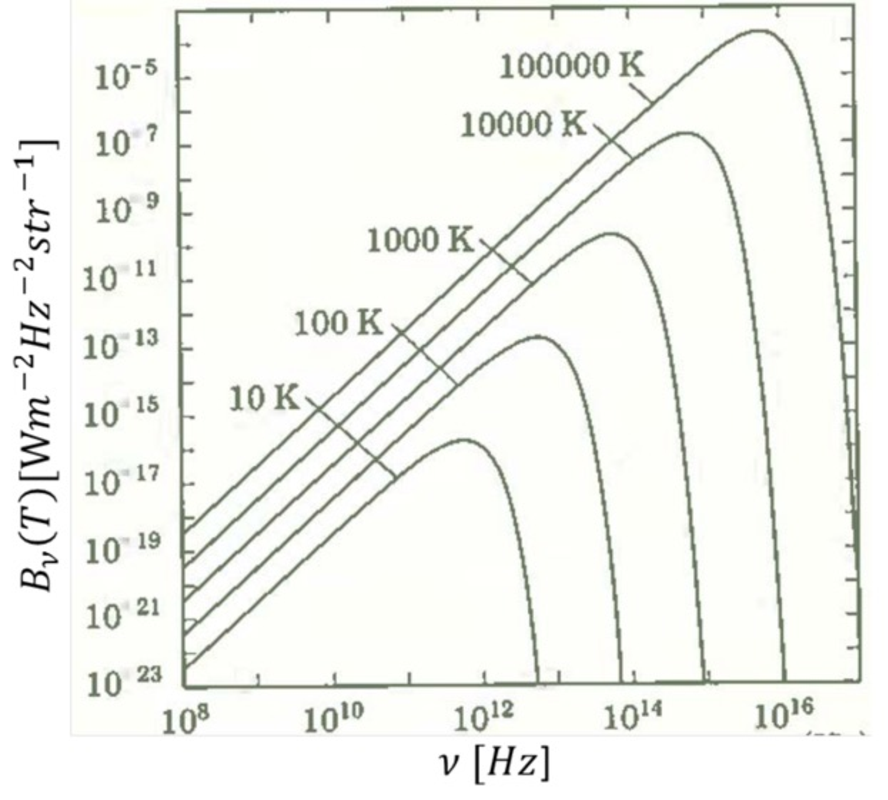
\includegraphics[width=\linewidth]{master_thesis_contents/master_thesis_fig/planck.pdf}
    \caption{Planckの放射式(~\cite{ito2017master}より引用)}
    \label{fig:planck}
\end{figure}
このように黒体温度と電波強度は比例の関係になり、大気分子からの電波強度を黒体の温度に換算することが可能である。
具体的には常温黒体(典型値として$300\, \mathrm{K}$)と液体窒素で冷却された黒体($77\, \mathrm{K}$)からの電波放射を受信機に入れることにより電波強度と黒体温度を対応させる。
\begin{figure}[htbp]
    \centering
    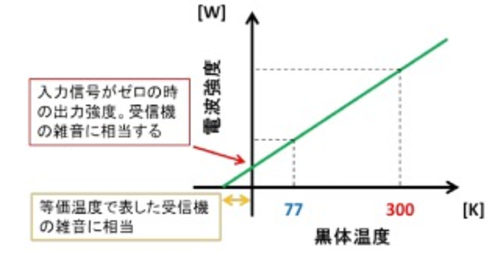
\includegraphics[width=\linewidth]{master_thesis_contents/master_thesis_fig/calibration.pdf}
    \caption{電波強度のキャリブレーションの様子(~\cite{ito2017master}より引用)}
    \label{fig:calibration}
\end{figure}
図\ref{fig:calibration}に示す直線が電波強度と黒体温度の対応を示している。
また直線の$y$切片の値は受信機雑音を示し、$x$切片の値の絶対値は受信機雑音を黒体温度で表した値となる。


次に、電波強度の補正に用いる光学的厚みについて述べる。
また、図\ref{fig:spectrometer_schema}に示す通りに、成層圏よりも高い高度を分子スペクトルを地上で観測する際には、下層大気(主に対流圏)を通過してきた電波を観測することになる。
そのため、下層大気に含まれる水蒸気や雲の放射や吸収の影響を考慮に入れるため、光学的厚みという概念を導入する。


光学的厚みがどのように電波強度に影響するかを述べる。
図\ref{fig:depth_dx}のように、厚さ$dx$の大気層があり、図の左から強度$T$の電波が入射したときを考える。
大気層で吸収および放射の影響を受けて、図の右に出てくる電波強度は$T+dT$で表される。
\begin{figure}[htbp]
    \centering
    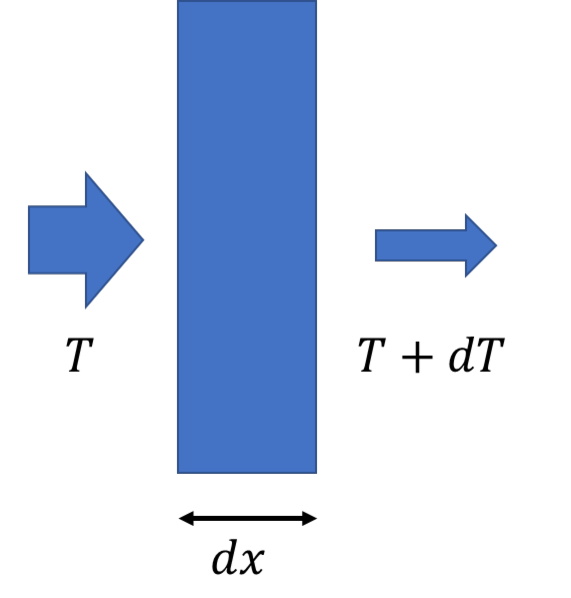
\includegraphics[width=\linewidth]{master_thesis_contents/master_thesis_fig/depth_dx.pdf}
    \caption{厚さ$dx$の大気層を通過する電波強度の模式図}
    \label{fig:depth_dx}
\end{figure}
このとき、吸収と自己放射を表す式は、$\kappa$を吸収係数、$j$を放射係数とすると
\begin{equation}
    dT = -\kappa T dx + j dx
    \label{eq:absorption_selfemission_1}
\end{equation}
となる。
次に光学的厚み(一般的に$\tau$で表す)を導入する。$\tau$は、
\begin{equation}
    \tau = \int_{0}^{x} \kappa dx' + j dx
\end{equation}
もしくは
\begin{equation}
    d\tau = \kappa dx
\end{equation}
と表され、これを用いて式\refeq{eq:absorption_selfemission_1}を書き換えると
\begin{equation}
    \frac{dT}{d\tau} = -T + \frac{j}{\kappa}
    \label{eq:absorption_selfemission_4}
\end{equation}
となる。
次に、式\refeq{eq:absorption_selfemission_4}の第2項において、熱平衡状態ではキルヒホッフの法則より
\begin{gather}
    \frac{j}{\kappa}
    = \frac{2h\nu^3}{c^2} \cdot \cfrac{1}{\exp\left(\cfrac{h\nu}{kT}-1\right)}
    \equiv I_\nu
    = T_\mathrm{sky} \\
    % I_\nu :電波強度、T_{sky}:大気からの熱放射、c:光速、k:Boltzmann定数 \notag \\
    % h:Planck定数、\nu :周波数、T:黒体温度 \notag
    T_\mathrm{sky}:大気からの熱放射 \notag
    \label{eq:absorption_selfemission_5}
\end{gather}
が成り立つ。
これを利用して式\refeq{eq:absorption_selfemission_5}より式\refeq{eq:absorption_selfemission_4}の解を求めると、
\begin{gather}
    T = T_0\exp\left(-\tau\right) + T_\mathrm{sky}\left(1-\exp\left(-\tau\right)\right) + T_\mathrm{sys} \\
    T_0 :大気分子からの電波強度、T_\mathrm{sky}:受信機雑音 \notag
    \label{eq:absorption_selfemission_6}
\end{gather}
となる。
これは、第1項が下層大気による電波吸収を考慮した(より上層にある)観測対象の分子からの電波強度、第2項は下層大気の熱放射を表している。
実際の観測で得られるスペクトルデータとしては第1項が図\ref{fig:spectum_thermalnoise}における橙色の成分、第2項が青色の成分に対応する(実際には青色の成分に受信機雑音も含まれるが、その詳細はこの後述べる)。
\begin{figure}[htbp]
    \centering
    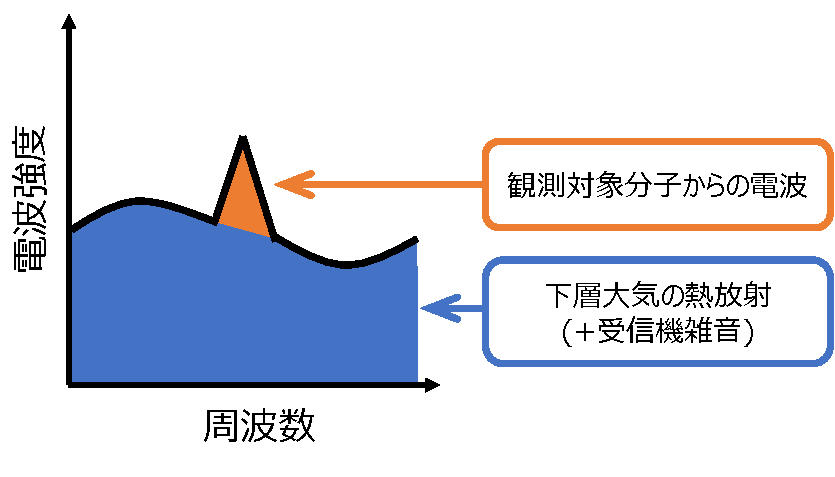
\includegraphics[width=\linewidth]{master_thesis_contents/master_thesis_fig/spectum_thermalnoise.pdf}
    \caption{スペクトルデータの強度を決める要素}
    \label{fig:spectum_thermalnoise}
\end{figure}
式\refeq{eq:absorption_selfemission_6}の左辺$T$が観測データから直接的に得られる値であるが、我々が知りたい値は、もともとの放射強度である$T_0$であるので、$T_0$を知るためには光学的厚みによる補正が必要となるわけである。(光学的厚みの測定方法の詳細は後述する。)


観測対象の分子スペクトルを得るために、大気の熱放射と観測装置の受信機からのノイズによるオフセット成分を除去する必要があり、周波数スイッチング(以後FRSWとする)という手法を用いる(図\ref{fig:frsw_schema})。
\begin{figure}[htbp]
    \centering
    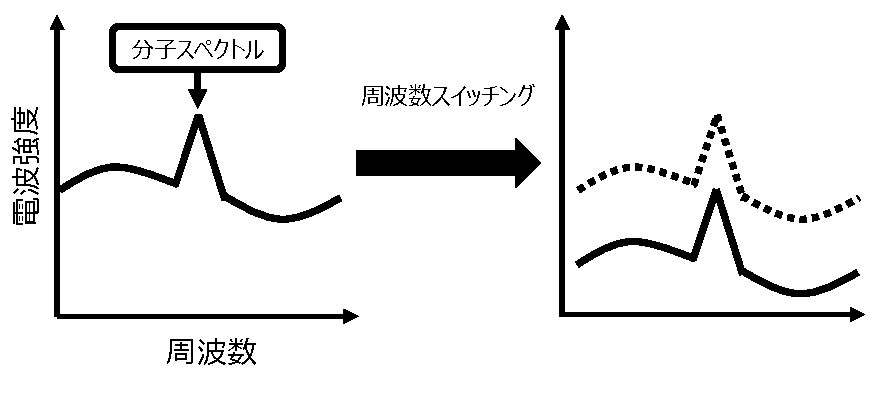
\includegraphics[width=\linewidth]{master_thesis_contents/master_thesis_fig/frsw_schema.pdf}
    \caption{周波数スイッチング(FRSW)の模式図}
    \label{fig:frsw_schema}
\end{figure}
FRSWによるオフセット成分の除去はおおまかなものであり、本研究では弱いスペクトルを検出する必要があるため、さらに細かくオフセット成分を補正する必要があるが、その詳細は\ref{sec:correction_baselinefitting}節で述べる。
本研究では、FRSWに加えて周波数折返し処理という解析方法を用いることで、オフセット成分を除去するとともに、スペクトルデータの信号対雑音比(S/N比)を向上させている。
\begin{figure}[htbp]
    \centering
    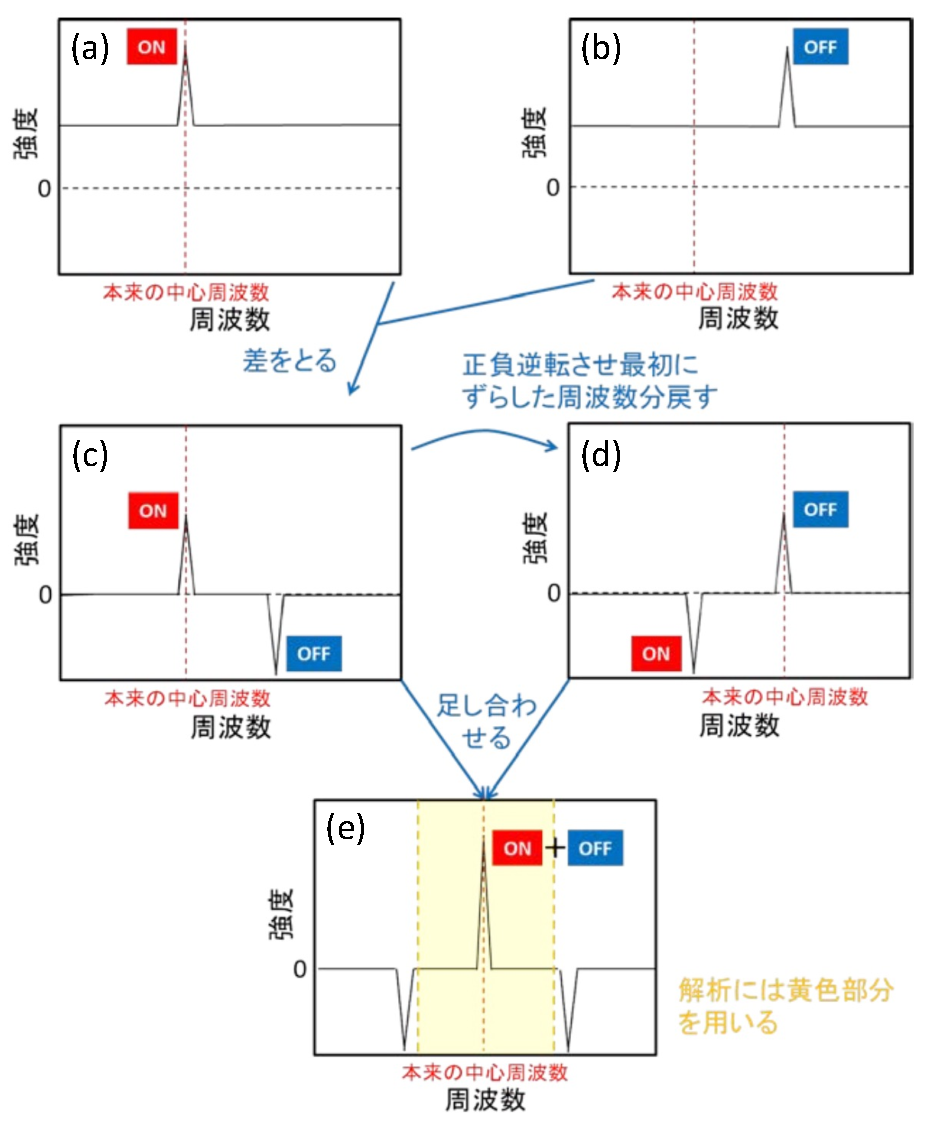
\includegraphics[width=\linewidth]{master_thesis_contents/master_thesis_fig/frsw_process.pdf}
    \caption{周波数スイッチングと周波数折り返し処理の概要(\cite{ito2017master}より引用)}
    \label{fig:frsw_process}
\end{figure}
まず、元となる最初に取得されたデータを図\ref{fig:frsw_process}(a)に示す。
次に、本来の局部発振器周波数から$\Delta f$だけ周波数をずらしたデータを取得する(図\ref{fig:frsw_process}(b))。
解析では、まず(a)から(b)を差し引いたデータを作成する(図\ref{fig:frsw_process}(c))。
これにより、(a)から(b)に共通に乗っていたオフセット成分が差し引かれる。
さらに(c)を上下反転して、ずらした周波数$\Delta f$を戻した(d)を作成する。
この(d)と(c)のデータを足し合わせて2で割る処理をする(周波数折り返し処理)。
(a)と(b)で取得された輝線スペクトルのデータは独立なものなので、この処理をすることによって、S/N比が$\sqrt{2}$倍向上する(図\ref{fig:frsw_process}(e))。
最終的に得られる分子スペクトルは図\ref{fig:frsw_process}(e)中の黄色で囲まれたところのみを使う。


次に、光学的厚みをどのように測定するかについて述べる。
光学的厚みの測定は図\ref{fig:opticaldepth_measurement}のように観測の間に行われており、トロムソの観測装置ではおよそ5分おきに測定されている。
% 昭和基地も同じなのか?
% 図を改良する必要あり
\begin{figure}[htbp]
    \centering
    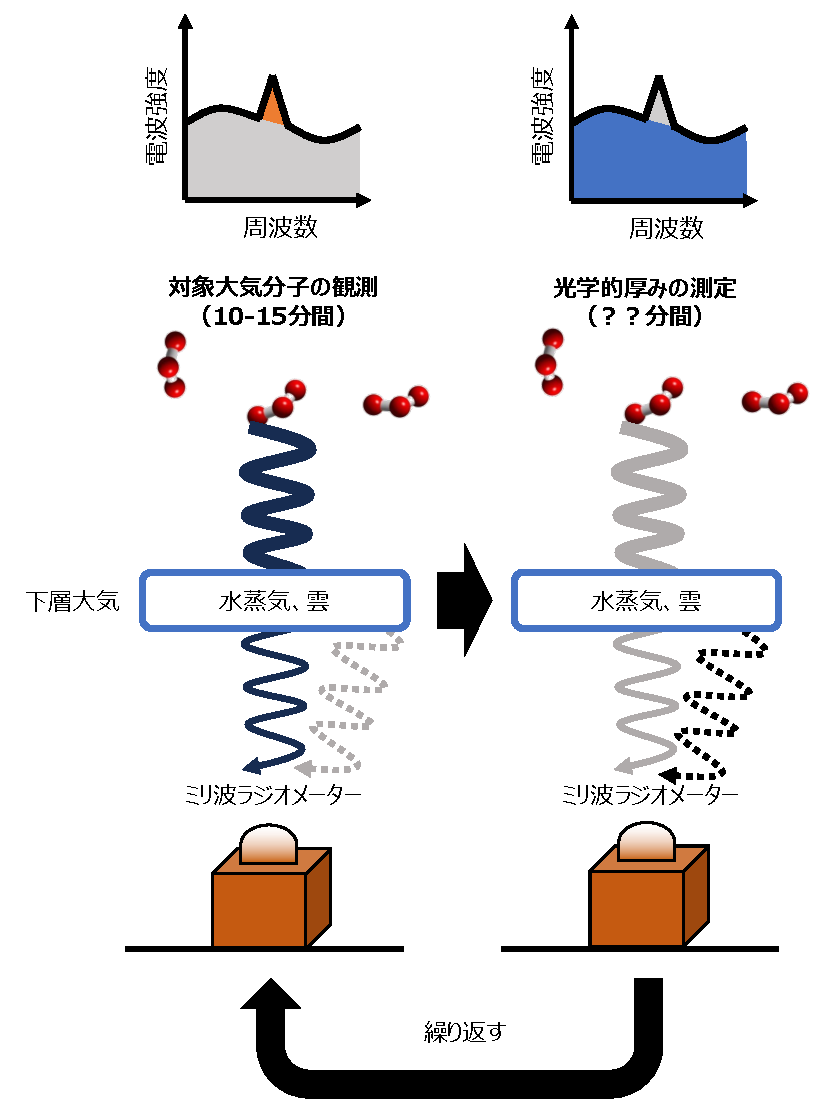
\includegraphics[width=\linewidth]{master_thesis_contents/master_thesis_fig/opticaldepth_measurement.pdf}
    \caption{ミリ波観測と光学的厚み$(\tau)$の測定の流れ}
    \label{fig:opticaldepth_measurement}
\end{figure}
測定された光学的厚みは直前に観測された電波強度のデータの補正に用いられる。
光学的厚みの測定についてはSky tippingと呼ばれる手法が用いられる。
まず関係式として、
\begin{gather}
    \begin{cases}
        T_z = T_\mathrm{sky}\{ 1-\exp (-\tau \sec z) \} + T_\mathrm{sys} \\
        T_\mathrm{obs\_ hot} = T_\mathrm{hot} + T_\mathrm{sys}
    \end{cases}
    \label{eq:opticaldepth_measurement} \\ \notag
    z :観測する角度の天頂角 \\ \notag
    T_\mathrm{z} :天頂角zでの分子スペクトルを含まない周波数の信号強度 \\ \notag
    % T_{sky} :大気からの熱放射、T_{sys} :観測装置の自己雑音温度 \\ \notag
    T_\mathrm{obs\_ hot} :常温黒体を見たときの輝度温度 \\ \notag
\end{gather}
ここで、$T_\mathrm{sky} = T_\mathrm{hot}$と仮定し式\refeq{eq:opticaldepth_measurement}の2式の差をとって両辺対数をとると
\begin{equation}
    \ln \left( T_{obs\_ hot} - T_z \right)  = \ln T_{obs\_ hot} - \tau \sec z
    % \ln \( T_{obs\_ hot} - T_z \) = \ln T_{obs\_ hot} - \tau \sec z
\end{equation}
この式は$y=ax$のような一次関数になっているため、左辺$\ln \left( T_\mathrm{obs\_ hot} - T_z \right)$を縦軸、$\sec z$を横軸としたプロットを作成すると図\ref{fig:opticaldepth_slope_tau}のようになることがわかる(プロットデータは観測装置の回転鏡により$z$の値を変えている)。
これらのプロットに対して一次の近似直線を引いたとき、その直線の傾きが光学的厚みに負の符号をつけたものと対応する。
以上より、光学的厚みを観測的に求めることができる。
\begin{figure}[htbp]
    \centering
    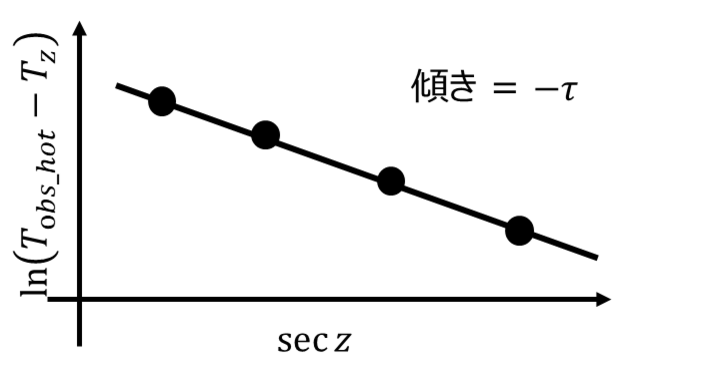
\includegraphics[width=\linewidth]{master_thesis_contents/master_thesis_fig/opticaldepth_slope_tau.pdf}
    \caption{光学的厚み$\tau$を求めるためのプロットデータ}
    \label{fig:opticaldepth_slope_tau}
\end{figure}
トロムソの観測装置で実際に測定している$\sec z$の値は表\ref{tb:secz_zdeg}のようになっている。
ここでは、それに対応した天頂角$z$と仰角の値も示す。
\begin{table}[htbp]
    \centering
    \caption{$\sec z$と天頂角$z\ [ \deg ]$と仰角$[ \deg ]$との対応}
    \label{tb:secz_zdeg}
    \setlength{\belowcaptionskip}{5mm}
    \begin{tabular}{ccc}
    \hline
    $\sec z$ & 天頂角 $z\ [ \deg ]$ & 仰角$[ \deg ]$ \\ \hline
    1.46     & 47                & 43           \\ \hline
    1.83     & 57                & 33           \\ \hline
    2.28     & 64                & 26           \\ \hline
    2.79     & 69                & 21           \\ \hline
    \end{tabular}
\end{table}
次の\ref{sec:mm_tromsoe}節と\ref{sec:mm_syowa}節では、それぞれ観測を立ち上げた時期と設置されてきた分光計の概要を述べる。トロムソと昭和基地で設置された分光計の仕様を表\ref{tb:spectrometer_spec}に示す。
% Single frequencyは「単周波数分光計」と訳せばいいのか?
\begin{table}[htbp]
    \centering
    \caption{トロムソ(1段目)と昭和基地(2段目)で設置された分光計の仕様}
    \label{tb:spectrometer_spec}
    \setlength{\belowcaptionskip}{5mm}
    \resizebox{\columnwidth}{!}{%
    \begin{tabular}{ccccc}
    \hline
    &
        期間 &
        FrontEnd &
        BackEnd &
        観測対象の分子 \\ \hline
    単周波数分光計 &
        \begin{tabular}[c]{@{}c@{}}2012年1月 –\\ 2020年8月\end{tabular} &
        \begin{tabular}[c]{@{}c@{}}1 Double sideband\\ PCTJ  SiS mixer\end{tabular} &
        \begin{tabular}[c]{@{}c@{}}FFT 分光計\\ 帯域 $\sim$1 GHz\\ 分解能 $\sim$61 kHz\end{tabular} &
        \begin{tabular}[c]{@{}c@{}}\ce{NO}, \ce{O3} \\ (分子同時観測不可能)\end{tabular} \\ \hline
    % Multi-freq. Phase 1 &
    %     \begin{tabular}[c]{@{}c@{}}2020年11月 – \\ 2021年2月\end{tabular} &
    %     \begin{tabular}[c]{@{}c@{}}2 Single sideband\\ PCTJ SIS mixers\end{tabular} &
    %     \begin{tabular}[c]{@{}c@{}}FFT 分光計\\ 帯域 $\sim$1GHz\\ 分解能 $\sim$61 kHz\end{tabular} &
    %     \begin{tabular}[c]{@{}c@{}}\ce{NO}, \ce{O3}, \ce{CO}, \ce{HO2} \\ (分子同時観測可能)\end{tabular} \\ \hline
    % Multi-freq. Phase 2 &
    %     \begin{tabular}[c]{@{}c@{}}2021年3月 –\\ 2022年1月\end{tabular} &
    %     \begin{tabular}[c]{@{}c@{}}1 Single sideband\\ PCTJ SIS mixers\end{tabular} &
    %     \begin{tabular}[c]{@{}c@{}}FFT 分光計\\ 帯域 $\sim$2 GHz\\ 分解能 $\sim$61 kHz\end{tabular} &
    %     \begin{tabular}[c]{@{}c@{}}\ce{NO}, \ce{O3}, \ce{HO2} \\ (分子同時観測可能)\\ (due to oscillator damage)\end{tabular} \\ \hline
    多周波数分光計 &
    % 多周波数分光計 Phase 3 &
        2022年7月 – &
        \begin{tabular}[c]{@{}c@{}}2 Single sideband\\ series-array SIS mixers\end{tabular} &
        \begin{tabular}[c]{@{}c@{}}FFT 分光計\\ 帯域 $\sim$2.5 GHz\\ 分解能 $\sim$76 kHz\end{tabular} &
        \begin{tabular}[c]{@{}c@{}}\ce{NO}, \ce{O3}, \ce{CO}, \ce{NO2}, \ce{HO2}\\ (分子同時観測可能)\end{tabular} \\ \hline
    \end{tabular}
    }
\end{table}
% \afterpage{\clearpage}
\clearpage

\section{Troms\o , Norway(69.35\textdegree N, 19.14\textdegree E)}
\label{sec:mm_tromsoe}
% \begin{itemize}
%     \item 観測立ち上げが行われた背景
%     \item いつ観測立ち上げが行われたか
%     \item 分光計の概要(とくに帯域について)
% \end{itemize}
\ref{sec:intro_privious}節で述べた、ミリ波分光観測において夏に短期変動の観測ができないという課題を解決するためには、北極域において同様の観測を実施することにより、両極域で\ce{NO}の同時モニタリングをすることが必要である。
両極において日照時間の長さは真逆の関係になっており、一方の極が夏期ならもう一方の極は冬期になる。
したがって、光化学反応の影響を強く受ける夏期ではわからない場合に、同時期のもう一方の冬期の極でデータを取得して比較することで、高エネルギー電子の降り込み(EPP: Energetic Electron Precipitation)による短期間変動を定量的に切り分けることができると考えた。
そこで我々は、北極域での観測拠点としてノルウェーのトロムソにあるEISCAT(European Incoherent Scatter)レーダー観測所に、2015年から2016年にかけて新たな観測装置を設置した~\cite{ito2017master}。
トロムソは南極の昭和基地とおよそ地磁気緯度が同じであるため、大きなEPPが起きると同時に影響を受けると期待できる。
観測所を利用することで、観測立ち上げのために新たにインフラを整備する必要がないという利点があるほか、EISCATレーダーの観測によって得られる電子密度などのデータを用いて、電子降り込みに関する情報と比較することができるということも重要である。
トロムソはミリ波地上観測にとってははじめての観測地であるため、周囲の電波環境や新たな観測装置の特性は明らかではなく、実際にどのような質のデータが取れるのかということの確認が必要である。
そのため、取得データを科学的研究に最大限に活用するためには、まずはデータの傾向を精査する必要がある。
そして、その傾向を把握した上で、データのスクリーニング(特定の条件を設定し、全体のデータから解析に用いることができるデータのみを選別)をする必要がある(詳細は\ref{sec:screening_opticaldepth}節と\ref{sec:screening_spectralnoise}節にて述べる)。


\section{Syowa, Antarctic(69.00\textdegree S, 39.85\textdegree E)}
\label{sec:mm_syowa}
% \begin{itemize}
%     \item いつ観測立ち上げが行われたか
%     \item 過去の分光計の概要(とくに帯域について)
%     \item 多周波数分光計の設置
% \end{itemize}
南極・昭和基地では2011年に観測装置が立ち上げられ、現在まで観測が続けられている。
% 立ち上げが2011年?観測開始が2012年?
% 分光計は4つすべて用いられた?
昭和基地では\ce{O3}と\ce{NO}の同時観測を目指すため、多周波数分光計が設置されている。
今回用いた分光計は2022年7月より定常観測を行っており、分光帯域は従来の分光計と比較して$1\ GHz$から$2.5\ GHz$まで広がった(表\ref{tb:spectrometer_spec})。
帯域が広がったことにより観測できる\ce{NO}の輝線スペクトルの本数を増やすことができた。トロムソに設置されている分光計では2本の輝線スペクトルが観測できたが、昭和基地では6本の輝線スペクトルを観測することができた。
現在観測できる\ce{NO}の輝線スペクトル例を図\ref{fig:NO_spectr}に示す。
\begin{figure}[htbp]
    \centering
    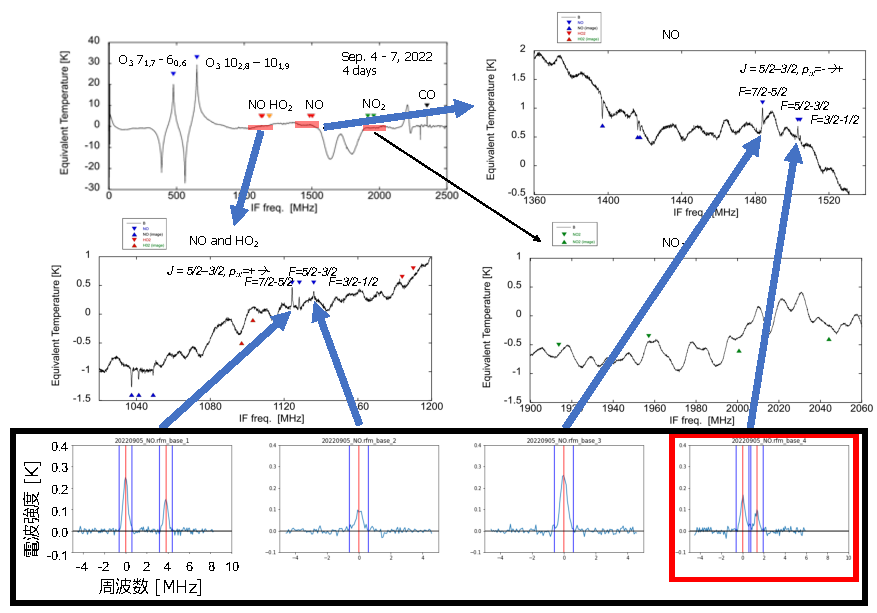
\includegraphics[width=\linewidth]{master_thesis_contents/master_thesis_fig/NO_spectr.pdf}
    % \caption{$\scriptstyle \mbox{昭和基地で現在観測できる6本の\ce{NO}輝線スペクトル} \scriptstyle
    % \mbox{(黒枠。赤枠はトロムソで観測できる2本の輝線スペクトル)}$}
    \caption{\protect 昭和基地で現在観測できる6本の\ce{NO}輝線スペクトル \linebreak
    (黒枠。赤枠はトロムソで観測できる2本の輝線スペクトル)}
    \label{fig:NO_spectr}
\end{figure}
\ce{O3}の輝線スペクトルと比較すると\ce{NO}の輝線スペクトルはとても微弱である。
そのため、どのデータが解析に用いることができるかスクリーニングを行い、電波強度の補正を行うことが重要となってくる。
詳細は\ref{ch:mm_analysis}章で述べていく。


% \chapter{ミリ波観測解析手法}
\chapter{ミリ波観測解析手法}
\label{ch:mm_analysis}
% 解析のフローチャートについて解、全体の解析の流れをしめす
% その背景を述べる(NOスペクトルの強度が微弱であることを含める)
\ref{ch:mm_obs}章で述べたように、トロムソは我々にとっては観測自体がはじめての場所であり、昭和基地においては分光計を更新してからはじめての観測である。
そのため、それぞれ観測装置立ち上げ後に行われたテスト観測のデータを1つずつ精査した。
また、\ref{sec:mm_syowa}節の図\ref{fig:NO_spectr}で示したように\ce{NO}の輝線スペクトルはとても微弱である。
そのため、S/N比がよい状態で輝線スペクトルを抽出する必要がある。
今回、\ce{NO}の柱密度の導出をするにあたって、スクリーニング(特定の条件を設定し、全体のデータから解析に用いることができるデータのみを選別)と電波強度の補正を行った。
ミリ波分光に関する装置は市販されていないため観測装置は自作となっており、その関係でスクリーニング、電波強度の補正に関わるプログラムは自ら作成した。
スクリーニングと電波強度の補正については、以下のようにそれぞれ2つの観点から行った。
\begin{itemize}
    \item スクリーニング
    \begin{itemize}
        \item 光学的厚みデータを用いたスクリーニング(\ref{sec:screening_opticaldepth}節)
        \item NOスペクトルデータに含まれるノイズによるスクリーニング(\ref{sec:screening_spectralnoise}節)
    \end{itemize}
    \item 電波強度の補正
    \begin{itemize}
        \item 光学的厚みデータの補正(\ref{sec:correction_opticaldepth}節)
        \item NOスペクトルデータのベースラインの補正(\ref{sec:correction_baselinefitting}節)
    \end{itemize}
\end{itemize}
\ref{sec:screening_opticaldepth}節と\ref{sec:correction_baselinefitting}節までのスクリーニングを行った結果、解析期間についてトロムソでは2019年1月23日 - 2019年2月4日と2019年2月17日 - 2019年2月20日、南極・昭和基地では2023年3月22日 - 2023年3月30日となった。
\ref{ch:mm_analysis}節では、それぞれの手法について上記のように順番に述べていき、最後の\ref{sec:derive_columndensity}節では柱密度の導出手法について述べる。

\section{光学的厚みデータを用いたスクリーニング}
\label{sec:screening_opticaldepth}

\ref{sec:mm_obs}節で述べたように、ミリ波分光計を用いた地上観測では下層大気による影響を受けるため、光学的厚みの測定データを用いてこの影響を取り除く必要がある。
したがって、光学的厚みの測定データは観測データに対して充分に安定していなければならない。
図\ref{fig:optical_depth_tromsoe}に示しているデータは、トロムソの観測装置立ち上げ後行われたテスト観測に測定された光学的厚みの時間変化を表したものである。
\begin{figure}[htbp]
    \centering
    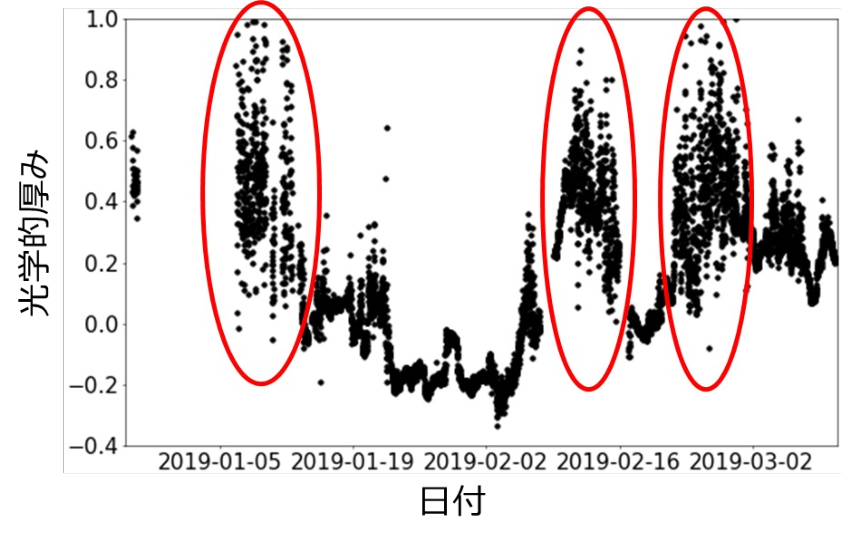
\includegraphics[width=\linewidth]{master_thesis_contents/master_thesis_fig/optical_depth_tromsoe.pdf}
    \caption{トロムソでの光学的厚み測定データの時間変化(~\cite{goto2021bachelor}より引用)}
    \label{fig:optical_depth_tromsoe}
\end{figure}
比較的値が安定している時期と、値が大きくばらついて安定していない時期がある(例として赤丸で示す)。
この赤丸で示された時期は、光学的厚みの典型値(たとえば南極昭和基地ではおよそ$0.1-0.4$の範囲の値をとる)とは大きく外れている。
さらに、このように短時間での値の変動が大きい場合は、それぞれ光学的厚みが測定された時間の間で下層大気の影響が一様でないことになる。
そのため、測定された光学的厚みの値を用いて、光学的厚みが測定された時間の間に観測された電波強度の補正をするには適さないと考えられる。
そこで、観測データの強度の補正に使用できる光学的厚みデータを判別するために、まず光学的厚みデータのスクリーニングを行うことを考える。
このスクリーニングで残った期間のNOスペクトルデータを後の解析に用いることとする。
判別方法としては、1日ごとにデータを区切りそれぞれの日の範囲で分散を計算し、その分散が$0.005$以下の値の日をとるデータを使用することとし、これを観測データのスクリーニングの条件として使用した。
この条件を設定することで、光学的厚みの変動が大きい日のデータを除去することができる。
分散の閾値を0.005としたのは図\ref{fig:optical_depth_tromsoe}のデータを目視し、値が安定していると判断した$2019年1月23日 - 2019年2月4日$の分散がいずれも0.005以下であったため、このように設定した~\cite{goto2021bachelor}。
南極・昭和基地の解析においても同条件でスクリーニングを行った。

\section{NOスペクトルデータに含まれるノイズによるスクリーニング}
\label{sec:screening_spectralnoise}

NOスペクトルデータにおいて、解析に使うことのできない質の悪いデータを事前にスクリーニングすることを考える。
トロムソの観測期間の全取得データを精査した結果、ノイズを含むスペクトルデータにおいて、スパイク状のノイズを含むデータと全体的にノイズを含むデータの2種類に大別できることがわかった~\cite{goto2021bachelor}。
スパイク状のノイズを含むデータと全体的にノイズを含むデータをそれぞれ判別する条件を考えることで、図\ref{fig:raw_spectrum}(a)のような質の良いデータのみを抽出することを目指す。
まず、NOスペクトルが存在する周波数を含むチャネル5000-10000の範囲のデータに対し2次曲線をフィッティングし、全体的にノイズがどれだけ含まれているか調べるために近似値に対する測定値の2乗平均誤差を計算した。
ここではチャネル5000-10000においてスペクトルデータの変動が二次関数的であったため、二次近似を用いている(図\ref{fig:raw_spectrum}(a)の赤線)。
\begin{figure}[htbp]
    \centering
    \begin{minipage}{0.33\linewidth}
        \centering
        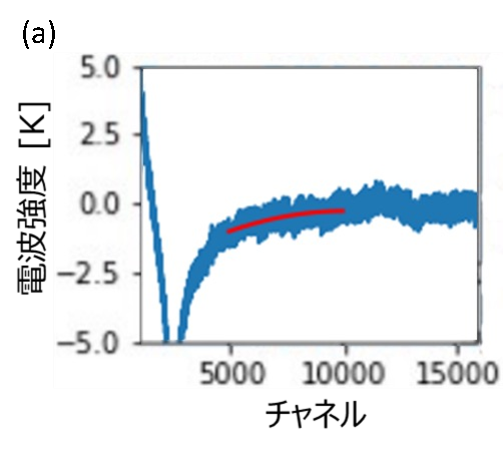
\includegraphics[width=\linewidth]{master_thesis_contents/master_thesis_fig/raw_spectrum_good.pdf}
        % \subcaption{解析に用いるために望ましい生データの一例($5000\, \mathrm{ch}$以下のデータは$239.093279\, \mathrm{GHz}$のオゾンの放射スペクトルデータがFRSWにより反映された結果、赤線は$5000-10000\, \mathrm{ch}$でのスペクトルデータの近似二次曲線を表す。~\cite{goto2021bachelor}より引用)}
        % \label{fig:raw_spectrum_good}
    \end{minipage}
    \begin{minipage}{0.6\linewidth}
        \centering
        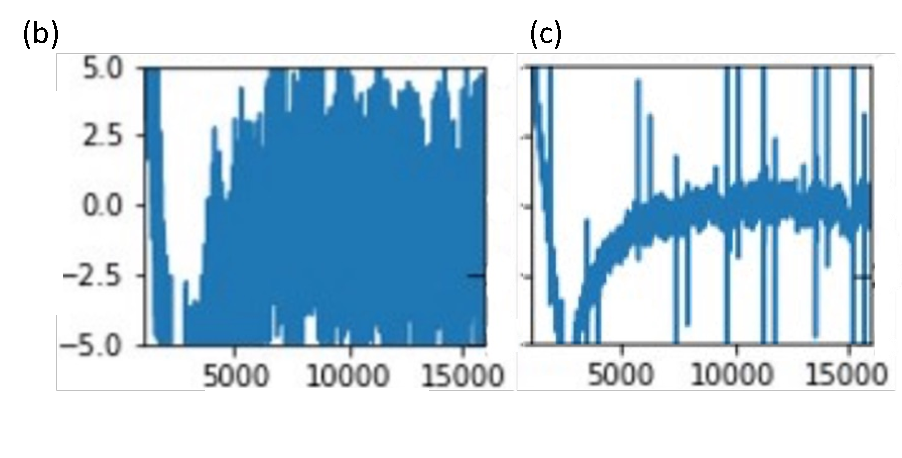
\includegraphics[scale=0.6]{master_thesis_contents/master_thesis_fig/raw_spectrum_bad.pdf}
        % \subcaption{スクリーニングしたいデータの例(左は全体的にノイズを含む例、右はスパイク状のノイズを含む例を表す)}
        % \label{fig:raw_spectrum_bad}
    \end{minipage}
    \caption{(a)解析に用いるために望ましい生データの一例($5000\, \mathrm{ch}$以下のデータは$239.093279\, \mathrm{GHz}$のオゾンの放射スペクトルデータがFRSWにより反映された結果、赤線は$5000-10000\, \mathrm{ch}$でのスペクトルデータの近似二次曲線を表す。)。(b)(c)スクリーニングしたいデータの例((b)は全体的にノイズを含む例、(c)はスパイク状のノイズを含む例を表す)。}
    \label{fig:raw_spectrum}
\end{figure}
これらの結果から、スクリーニング条件としては以下2つを設定した~\cite{goto2021bachelor}。
\begin{itemize}
    \item 2乗平均誤差の整数丸め値が0である
    \item チャネル5000-10000で強度の絶対値が$5\, \mathrm{K}$以上の値を含まない
\end{itemize}
1つ目の条件は、全体的にノイズを含むデータ(たとえば図\ref{fig:raw_spectrum}(b))を判別・除去することを意図しており、2つ目の条件はスパイク状のノイズを含むデータ(たとえば図\ref{fig:raw_spectrum}(c))を除去することを意図している。
設定したスクリーニング条件が妥当かどうかの検証は卒業研究~\cite{goto2021bachelor}にて行った。

\section{光学的厚みデータの補正(Troms\o)}
\label{sec:correction_opticaldepth}
\ref{sec:screening_opticaldepth}節の述べたように、不安定な光学的厚みのデータを除去するスクリーニングの結果によって、トロムソの観測データにおいて図\ref{fig:optical_depth_minus}のように期間A(2019年1月23日 - 2019年2月4日)、期間B(2019年2月17日 - 2019年2月20日)が残った。
しかし、期間Aにおいて光学的厚みが$-0.2$付近の負の値をとっていることがわかった(図\ref{fig:optical_depth_minus}の赤丸)。
\begin{figure}[htbp]
    \centering
    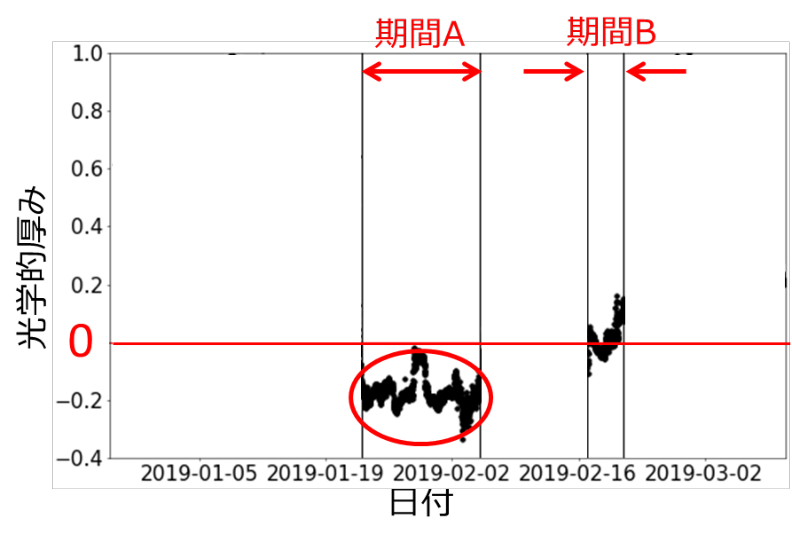
\includegraphics[width=\linewidth]{master_thesis_contents/master_thesis_fig/optical_depth_minus.pdf}
    \caption{トロムソにおいて負の値をとる光学的厚み(~\cite{goto2021bachelor}より引用)}
    \label{fig:optical_depth_minus}
\end{figure}
\ref{ch:mm_obs}章で述べた光学的厚みの算出方法のことを考えると、下層大気の光学的厚みの値が負の値を取ることはない。
そこでこの原因を調べたところ、光学的厚みを算出する際の各観測天頂角に対するプロットデータにおいて、もっとも観測天頂角が小さい($\sec z$が1番小さい)
ところのプロットデータが下に落ち込んでおり、それによって近似直線の傾きが変化してしまうことで、光学的厚みが負の値として計算されていることが分かった~\cite{goto2021bachelor}。
その模式図を図\ref{fig:optical_depth_slope_minus}、実際の測定データ例を図\ref{fig:optical_depth_measurement_good_bad}に示す。
\begin{figure}[htbp]
    \centering
    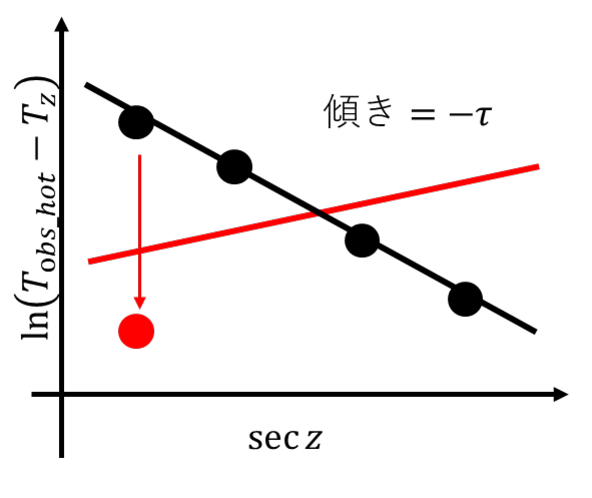
\includegraphics[width=\linewidth]{master_thesis_contents/master_thesis_fig/optical_depth_slope_minus.pdf}
    \caption{プロットデータの落ち込みによる光学的厚みの計算値の変化(プロットデータの落ち込みにより近似直線が黒線→赤線に変わり、直線の傾きが変わる)~\cite{goto2021bachelor}より引用。}
    \label{fig:optical_depth_slope_minus}
\end{figure}
\begin{figure}[htbp]
    \centering
    \begin{minipage}{0.41\linewidth}
        \centering
        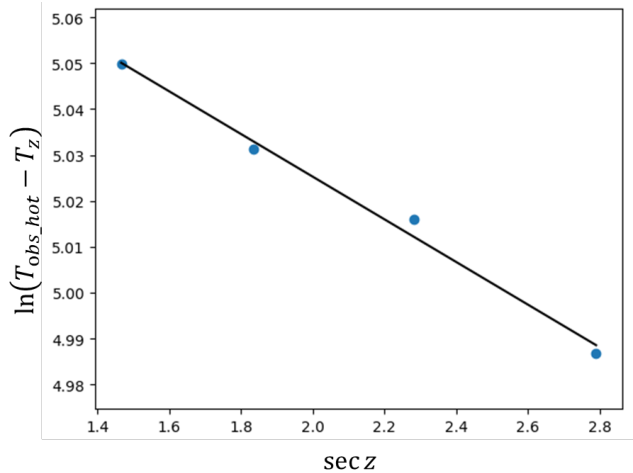
\includegraphics[width=\linewidth]{master_thesis_contents/master_thesis_fig/optical_depth_good.pdf}
    \end{minipage}
    \begin{minipage}{0.45\linewidth}
        \centering
        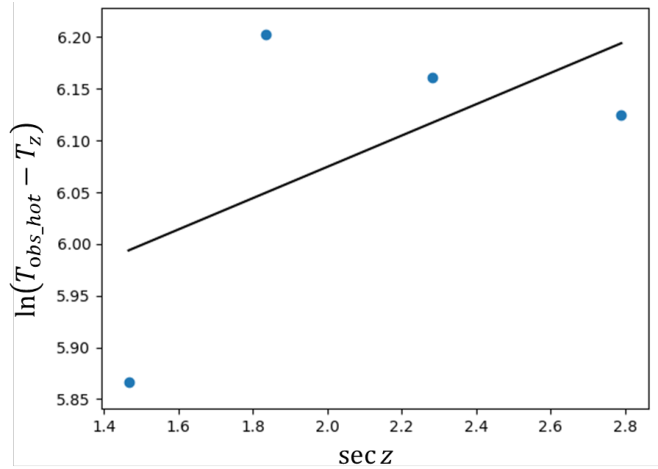
\includegraphics[scale=0.6]{master_thesis_contents/master_thesis_fig/optical_depth_bad.pdf}
    \end{minipage}
    \caption{(a)望ましいプロットデータの一例(2019年2月17日5時51分頃測定)。(b)プロットデータが落ち込んだ実際のデータの一例。(2019年1月23日0時5分頃測定)。黒線は近似直線を表す。~\cite{goto2021bachelor}より引用。}
    \label{fig:optical_depth_measurement_good_bad}
\end{figure}
さらに、そのプロットデータの落ち込みの原因を調べたところ、ちょうど光学的厚みの値が負の値となっている期間の終わりごろに、ミリ波観測装置のビームが通る側面の観測窓の上部に氷柱ができているのを見つけたという報告があり(図\ref{fig:icicles})、それが時期的に一致していることが分かった~\cite{goto2021bachelor}。
\begin{figure}[htbp]
    \centering
    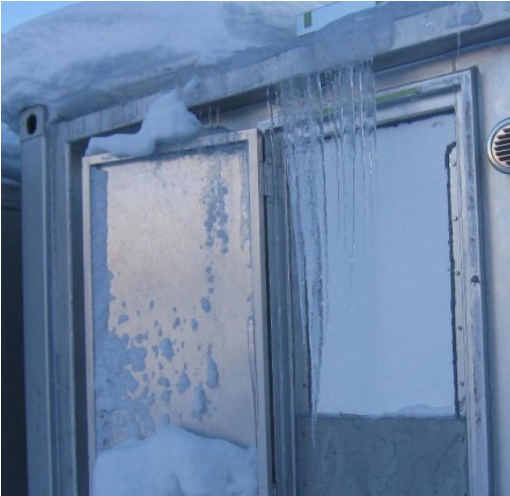
\includegraphics[width=\linewidth]{master_thesis_contents/master_thesis_fig/icicles.pdf}
    \caption{側窓にできた氷柱(~\cite{goto2021bachelor}より引用)}
    \label{fig:icicles}
\end{figure}
したがって、天頂角がもっとも小さい角度で測定された電波強度に影響を与えた可能性があると考え、そのデータを用いずに光学的厚みを測定し直し、光学的厚みの補正を行った。
設定した補正手法が妥当かどうかの検証は卒業研究~\cite{goto2021bachelor}にて行った。

\section{NOスペクトルデータのベースラインの補正}
\label{sec:correction_baselinefitting}
\ref{sec:screening_opticaldepth}節や\ref{sec:screening_spectralnoise}節によるスクリーニングで残った期間における\ce{NO}スペクトルデータについて積分を行う(積分時間はトロムソでは24時間、南極・昭和基地では12時間)。
これは昭和基地で行われた先行研究であるIsonoらによる研究~\cite{isono2014ground}より、1日程度の積分をすることで十分なS/N比で議論することができると考えたためである。
そして、観測データに含まれている\ce{NO}のスペクトルを検出するため、ベースラインの補正を行う。
ここでは、スペクトルの両端におけるデータを用いてバックグラウンドのベースラインを近似から求め、それを元のスペクトルから差し引くことによって、FRSWで除去しきれなかったオフセット成分や周波数特性のうねりなどをを除去した。
ベースラインの補正の模式図を図\ref{fig:baseline_correct_schema}に示す。
\begin{figure}[htbp]
    \centering
    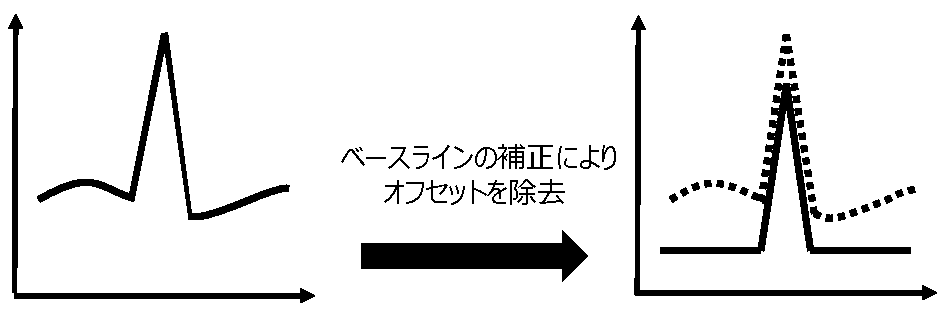
\includegraphics[width=\linewidth]{master_thesis_contents/master_thesis_fig/baseline_correct_schema.pdf}
    \caption{ベースライン近似を用いたベースラインの補正}
    \label{fig:baseline_correct_schema}
\end{figure}
ベースラインの近似に用いるデータは、図\ref{fig:baseline_range}の赤色で示したスペクトルの両端のそれぞれ$5\, \mathrm{MHz}$の範囲とした。
% 近似の範囲は、syowaだといくつ?
この範囲は、対象とするNOの放射スペクトル成分が含まれないと考えられる。
\begin{figure}[htbp]
    \centering
    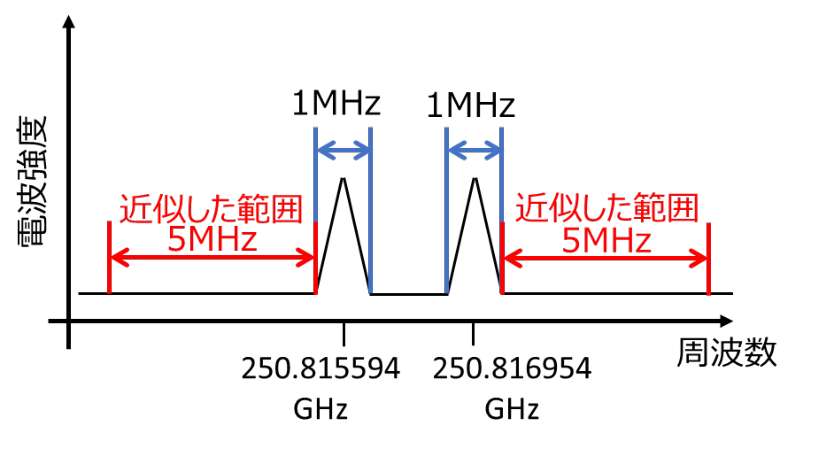
\includegraphics[width=\linewidth]{master_thesis_contents/master_thesis_fig/baseline_range.pdf}
    \caption{ベースラインを補正する元となる周波数の範囲(赤色で表示。青色は検出するスペクトルの幅を示している。例としてトロムソで用いた2本の輝線スペクトルの場合を示した。)}
    \label{fig:baseline_range}
\end{figure}
スペクトルデータのベースラインの特性の傾向が、図\ref{fig:baseline_curve}示す赤い曲線のような三次関数的な形であったので、ここでは三次関数で近似を行うことにした。
\begin{figure}[htbp]
    \centering
    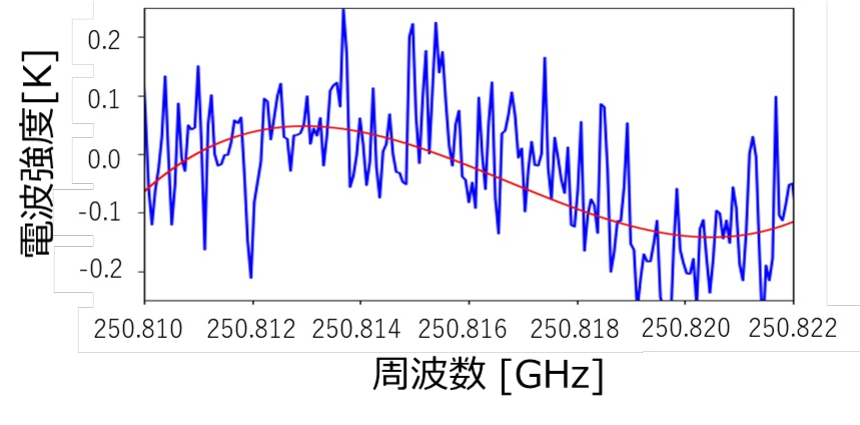
\includegraphics[width=\linewidth]{master_thesis_contents/master_thesis_fig/baseline_curve.pdf}
    \caption{三次関数的な形のベースライン(~\cite{goto2021bachelor}より引用)}
    \label{fig:baseline_curve}
\end{figure}
また、\ce{NO}の各スペクトル幅は$1\, \mathrm{MHz}$と仮定した。
このように仮定したのは対象の時期の日ごとのデータにおいて、放射スペクトルである三角の山状の幅の大きさがどの日のデータにおいてもおよそ$1\, \mathrm{MHz}$であることが確認できたためである(図\ref{fig:no_spectr_exp}にあるデータの一例において、スペクトル幅がおよそ$1\, \mathrm{MHz}$であることが確認できる)。
\begin{figure}[htbp]
    \centering
    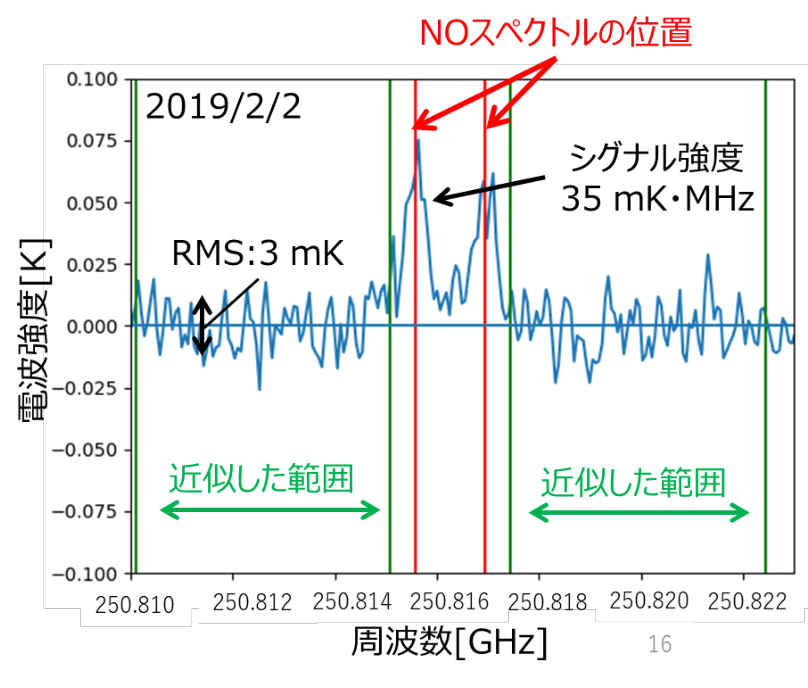
\includegraphics[width=\linewidth]{master_thesis_contents/master_thesis_fig/no_spectr_exp.pdf}
    \caption{スペクトルの検出の一例(赤線は検出するスペクトルがある周波数の位置、緑線はベースライン近似に用いたスペクトルデータの範囲を示す。~\cite{goto2021bachelor}より引用)}
    \label{fig:no_spectr_exp}
\end{figure}
\clearpage

\section{NO柱密度の導出}
\label{sec:derive_columndensity}
柱密度とは高度方向に密度を足し合わせたものであり、今回はスペクトルの線形から$70\, \mathrm{km}$以上に存在する\ce{NO}分子についてみたものとなる。
柱密度の導出においては先行研究~\cite{isono2014ground}を参考にして行った。
導出に用いた式は以下のようになる。
\begin{gather}
    N_{\mathrm{NO}} = A \times T_{\mathrm{atm}} \times \int T_{\mathrm{NO}}d\nu
    \label{eq:derive_columndensity} \\
    N_{\mathrm{NO}}:\ce{NO}の柱密度[\mathrm{cm^{-2}}]、A:線スペクトル強度係数[\mathrm{K^{-2}} \cdot \mathrm{MHz^{-1}} \cdot \mathrm{cm^{-2}}] \notag \\
    T_{\mathrm{atm}}:大気温度[\mathrm{K}]、\int T_{\mathrm{NO}}d\nu:\ce{NO}のスペクトル積分強度 \notag
\end{gather}
線スペクトル強度係数は輝線スペクトルの強度を知るための分子パラメーターで分子・周波数ごとに決まる値となる。
今回用いた\ce{NO}の輝線スペクトルにおけるそれぞれの線スペクトル強度係数については\ref{ch:mm_analysis}章の表\ref{tb:no_spectr_freq}に記載している。
大気温度については一様に$200\, \mathrm{K}$と仮定し、\ce{NO}が存在する領域においては光学的に薄いと仮定している。
誤差については\ref{sec:correction_baselinefitting}節で述べたベースライン近似の際に用いた範囲でのRMS(Root Mean Square)を用いて、式\refeq{eq:derive_columndensity}と同様の方法で求めた。
式を以下に示す。
\begin{gather}
    % N_{\mathrm{NO}} = A \times T_{\mathrm{atm}} \times T_{\mathrm{rms}} \\
    N_{\mathrm{NO}} = A \times T_{\mathrm{atm}} \times \int T_{\mathrm{rms}}d\nu \\
    T_{\mathrm{rms}}:\mathrm{RMS[K]} \notag
\end{gather}
% 式の記述は正しい?
また、柱密度をプロットするにあたって、はじめに柱密度の導出はそれぞれの輝線スペクトルについて行い(式\refeq{eq:derive_columndensity})、次に用いた輝線スペクトルの柱密度について平均を計算した。
柱密度の平均については、それぞれの輝線スペクトルの柱密度を導出する際に用いた線スペクトル強度係数によって重み付けをした。
線スペクトル強度係数による重み付けの平均の式を以下に示す。
\begin{gather}
    N_{\mathrm{avg}} = \left. \sum_{k} \frac{N_{k}}{\varepsilon_{k}} \middle/ \sum_{k} \frac{1}{\varepsilon_{k}} \right. \\
    N_{\mathrm{avg}}:\ce{NO}の平均柱密度、N_{\mathrm{k}}:一つの輝線スペクトルから導出した柱密度 \notag \\
    \varepsilon_{\mathrm{k}}:一つの輝線スペクトルから導出した柱密度の誤差 \notag
\end{gather}
また、柱密度の誤差についても以下のように同様に重み付けによる平均を計算した。
\begin{equation}
    \varepsilon_{\mathrm{avg}} = \left( \sum_{k} \frac{1}{\varepsilon_{k}} \right)^{-1}
    % \varepsilon_{\mathrm{avg}} = \left. 1 \middle/ \sum_{k} \frac{1}{\varepsilon_{k}} \right.
\end{equation}


% \chapter{結果}
\chapter{結果}
\label{ch:results}
\section{Troms\o , Norway}
\label{sec:results_tromsoe}
\section{Syowa, Antarctic}
\label{sec:results_syowa}


% \chapter{考察}
\chapter{考察}
% \label{ch:discussion}
\section{SOFIEデータによって導出されたNO柱密度との比較}
% \label{sec:comparison_sofie}
\section{高エネルギー電子の降込みとの比較}
% \label{sec:comparison_eep}


% \chapter{まとめ}
\chapter{まとめ}
% \label{ch:conclusion}


% \chapter*{謝辞}
\chapter*{謝辞}
% \label{ch:acknowledgement}


\bibliographystyle{junsrt}
\bibliography{master_thesis_ref}

\appendix
% \chapter{SOFIE衛星}
\chapter{SOFIE衛星}
% \label{app:sofie}

% \chapter{POES/MetOp衛星}
\chapter{POES/MetOp衛星}
% \label{app:poes}


\end{document}
